\begin{defnbox}\nospacing
    \begin{defn}[\hfill\exampleref{example:graph_visualization}\newline Torch Dynamo]\label{defn:torch_dynamo}\leavevmode\\
        Torch Dynamo is a JIT compiler that generates \textit{FX Graphs}\cref{defn:fx_graph} from Python bytecode.\\
        It uses the frame evaluation API in CPython to dynamically modify Python bytecode before execution.\\
        This modified python bytecode is then extracted into an FX Graph which can then be just-in-time compiled with a suitable backend.
        \begin{figure}[H]
            \vspace{-1em}
            \centering{
              \def\svgwidth{200pt}
              \resizebox{\linewidth}{!}{\begin{defnbox}\nospacing
    \begin{defn}[Torch Dynamo]\label{defn:torch_dynamo}\leavevmode\\
        Generates \textit{FX Graphs}\cref{defn:fx_graph} from Python bytecode.\\
        It uses the frame evaluation API in CPython to dynamically modify Python bytecode before execution.\\
        This modified python bytecode is then extracted into an FX Graph which can then be just-in-time compiled with a suitable backend.
        \begin{figure}[H]
            \vspace{-1em}
            \centering{
              \def\svgwidth{200pt}
              \resizebox{\linewidth}{!}{\begin{defnbox}\nospacing
    \begin{defn}[Torch Dynamo]\label{defn:torch_dynamo}\leavevmode\\
        Generates \textit{FX Graphs}\cref{defn:fx_graph} from Python bytecode.\\
        It uses the frame evaluation API in CPython to dynamically modify Python bytecode before execution.\\
        This modified python bytecode is then extracted into an FX Graph which can then be just-in-time compiled with a suitable backend.
        \begin{figure}[H]
            \vspace{-1em}
            \centering{
              \def\svgwidth{200pt}
              \resizebox{\linewidth}{!}{\begin{defnbox}\nospacing
    \begin{defn}[Torch Dynamo]\label{defn:torch_dynamo}\leavevmode\\
        Generates \textit{FX Graphs}\cref{defn:fx_graph} from Python bytecode.\\
        It uses the frame evaluation API in CPython to dynamically modify Python bytecode before execution.\\
        This modified python bytecode is then extracted into an FX Graph which can then be just-in-time compiled with a suitable backend.
        \begin{figure}[H]
            \vspace{-1em}
            \centering{
              \def\svgwidth{200pt}
              \resizebox{\linewidth}{!}{\input{pytorch_submodule/src/the_framework/graph_acquisition/figures/torch_dynamo.pdf_tex}}
            }
        \end{figure}
    \end{defn}
\end{defnbox}
\begin{notebox}[Note]\nospacing
    \begin{itemizenosep}
        \item Torch Dynamo maintains the eager-mode capabilities using guards to ensure the generated graphs are valid
    \end{itemizenosep}
\end{notebox}

%%% Local Variables:
%%% mode: latex
%%% TeX-command-extra-options: "-shell-escape"
%%% TeX-master: "../../../../../formulary"
%%% End:
}
            }
        \end{figure}
    \end{defn}
\end{defnbox}
\begin{notebox}[Note]\nospacing
    \begin{itemizenosep}
        \item Torch Dynamo maintains the eager-mode capabilities using guards to ensure the generated graphs are valid
    \end{itemizenosep}
\end{notebox}

%%% Local Variables:
%%% mode: latex
%%% TeX-command-extra-options: "-shell-escape"
%%% TeX-master: "../../../../../formulary"
%%% End:
}
            }
        \end{figure}
    \end{defn}
\end{defnbox}
\begin{notebox}[Note]\nospacing
    \begin{itemizenosep}
        \item Torch Dynamo maintains the eager-mode capabilities using guards to ensure the generated graphs are valid
    \end{itemizenosep}
\end{notebox}

%%% Local Variables:
%%% mode: latex
%%% TeX-command-extra-options: "-shell-escape"
%%% TeX-master: "../../../../../formulary"
%%% End:
}
            }
        \end{figure}
        \imp{Optimize a model}:
        \begin{mintlinebox}{python}
            optimized_model = dynamo.optimize()(|\texttt{\optc{model}}|)
        \end{mintlinebox}
        \imp{Obtain detailed information}:
        \begin{mintlinebox}{python}
            explanation, out_guards, graphs, ops_per_graph,
            break_reasons, explanation_verbose
            = dynamo.explain(f1, x, y)
        \end{mintlinebox}
    \end{defn}
\end{defnbox}
\begin{notebox}[Notes]\nospacing
    \begin{itemizenosep}
        \item \pythoninline{torch.compile} is a wrapper for \pythoninline{torch._dynamo.optimize()}
        \item One can also get info using logging:
    \begin{plaincodebox}[colback=notebox]{python}
        import logging
        dynamo.config.log_level = logging.INFO
        dynamo.config.output_code = True
    \end{plaincodebox}
    \end{itemizenosep}
\end{notebox}
\begin{sectionbox}[Why Torch Dynamo?\hfill\exampleref{example:data_dependent_control_flow,example:module_dependent_control_flow}]\nospacing
    \begin{wrapfigure}{r}{0.45\linewidth}
        \centering
        \vspace{-10pt}
        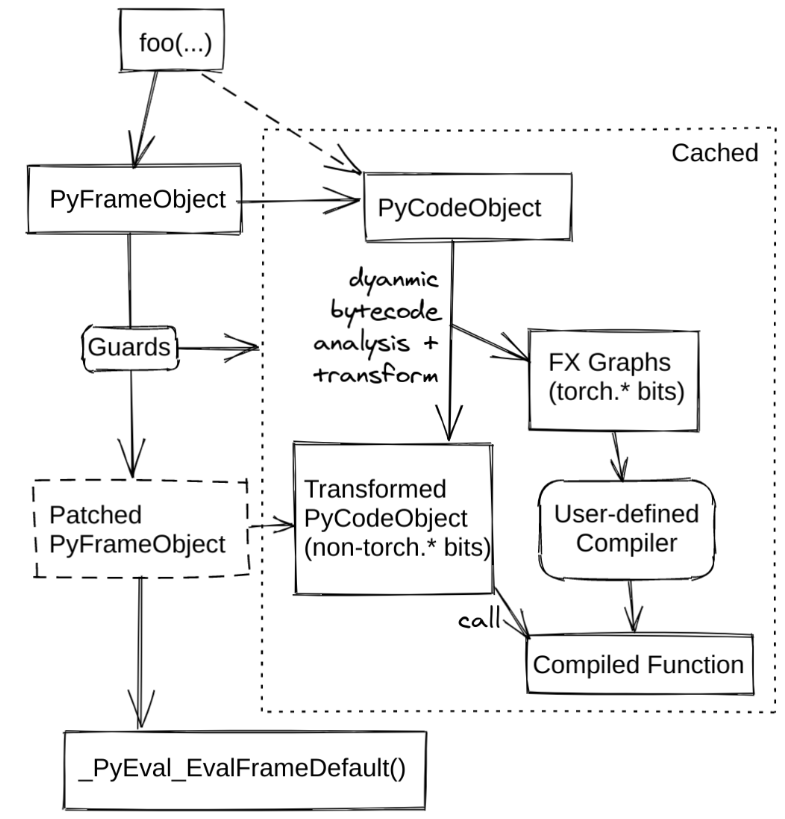
\includegraphics[width=\linewidth]{/home/pollakg/polybox/formularies/python/python/pytorch_submodule/src/the_framework/graph_acquisition/figures/torch_dynamo_partial_graphs.png}
    \end{wrapfigure}
    Why do we need Torch Dynamo if we have Torch Script \pythoninline{torch.jit} and
    Torch FX tracing \pythoninline{torch.fx.symbolic_trace}?\\
    \pythoninline{torch.fx.Graphs} are static Graphs, that cannot handle data-or module-dependent control flows.
    This is because \pythoninline{torch.fx.Graphs} and \pythoninline{torch.jit} use proxy/dummy variables to JIT compile/trace the graph.
    Torch Dynamo solves this problem by using guards and partial graphs.
\end{sectionbox}
\begin{corbox}\nospacing
    \begin{cor}[Partial Graphs]\label{cor:partial_graphs}\leavevmode\\
        Torch Dynamo allows to capture data-dependent control flows or non-PyTorch functions.
        It does so by breaking the computation graph whenever it encounters unsupported/un-tracable python code and letting the Python interpreter handle it, resuming
        execution afterwards.
        This is done using with the help of guards and leads to sets of \pythoninline{torch.fx.Graphs}.
    \end{cor}
\end{corbox}
\begin{defnbox}\nospacing
    \begin{defn}[Guards]\label{defn:guards}
        A criteria to check for Bytecode changes.
        Torch Dynamo caches modified Bytecode.
        When TorchDynamo receives a frame for evaluation, it checks if the objects referenced in the frame have changed using
        \textit{Guards}.
    \end{defn}
\end{defnbox}
\begin{notebox}[Note]\nospacing
      Guard allow Torch Dynamo to maintain the eager-mode capabilities to ensure the generated graphs are valid.
\end{notebox}
\paragraph{Options}\label{para:options}
\begin{optionsbox}\nospacing
    \begin{option}[\pythoninline{nopython=True}]\label{option:nopython_true}\leavevmode\\
        Forces full graphs (no partial graphs).
        This can be useful for:
        \begin{itemizenosep}
            \item extremly large scale training runs, that require pipeline parallelism, advanced shading
            \item Aggressive inference optimizer such as TensorRT or AITEmplate, that fuse much more aggresively
            \item Mobile training or inference
        \end{itemizenosep}
    \end{option}
\end{optionsbox}


%%% Local Variables:
%%% mode: latex
%%% TeX-command-extra-options: "-shell-escape"
%%% TeX-master: "../../../../../formulary"
%%% End:
